%!TEX root = ../Diploma.tex

\clearpage
\begin{section}{Политика Twitter в отношении спама}

\begin{subsection} {Структура Twitter}

  Twitter - социальная сеть, позволяющая пользователям писать сообщения, не превышающие 140 символов, которые могут быть увиденными и прокомментированными любым другим пользователем этой социальной сети. Структура Twitter представляет собой направленный граф, где пользователи — узлы, а ребра отражают отношения между ними.
  Некоторые определения:

  \textit{Твит (сообщение)}  - текст длиной до 140 символов, в котором могут содержаться ссылки, хэштеги и упоминания;

  \textit{Ретвит} - перепубликация твита, созданного другим пользователем;

  \textit{Хэштег} - специально зарезервированный символ <<\#>>, употребляемый перед словом, обозначающим принадлежность к определенной теме;

  \textit{Упоминание} - специально зарезервированный символ <<@>>, употребляемый перед именем пользователя;

  \textit{Тренд} - набор слов и хэштегов, популярность использования которых на определенный момент времени резко превышает остальные;

  В Twitter пользователь может формировать связь с другими пользователями путем подписки на их твиты. Простейший пример взаимоотношений пользователей показаны на Рисунке 1.
  \begin{figure}[ht!]
  \centering
  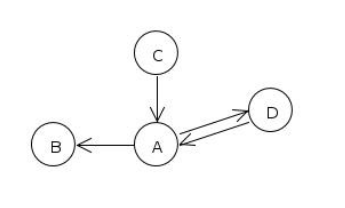
\includegraphics[width=0.4\textwidth]{pics/TwitterGraph}
  \caption{Пример взаимоотношения пользователей Twitter}
  \label{pic:TwitterGraph}
  \end{figure}

\end{subsection}
\begin{subsection}{Распространенность спама в Twitter}
Результаты исследований показывают, что более 3\% сообщений в Twitter являются спамом \cite{Kelly}, \cite{Wang}, около 8\% всех ссылок указывают на вредоносный контент \cite{Grier}. Также сообщается, что более 90\% всех спамовых сообщений содержат ссылки \cite{Benevenuto}.

В силу ограниченности длины статуса 140 символами
спамеры распространяют вредоносный контент преимущественно
посредством ссылок. Twitter трансформирует все ссылки
с помощью собственного сервиса по сокращению URL,
что позволяет спамерам не затрачивать дополнительных усилий
на маскировку источника.
В основной массе исследований приводятся описания
следующих выявленных стратегий спамеров:
\begin{enumerate}
\item Спам в отношении пользователей,
подписанных на спамера
(любой твит пользователя автоматически появляется в
новостной ленте его подписчиков) \cite{Vasumathi}, \cite{Kurt};
\item Использование упоминаний
(твит с упоминанием пользователя появляется в новостной
ленте упомянутого, независимо от того,
является он подписчиком спамера или нет) \cite{Kurt};
\item Покупка подписчиков с целью создания видимости благонадежной репутации аккаунта \cite{Vasumathi},
покупка ретвитов \cite{Grier};
\item Спам в отношении пользователей, чьи твиты содержат слова релевантные проводимой спам-кампании
\cite{Vasumathi};
\item Использование в твитах популярных поисковых слов (техника напоминает SEO) \cite{Kurt};
\item Эксплуатация хэштегов популярных тем \cite{Kurt}, \cite{Martinez}, создание спамерских тем \cite{Grier};
\item Изменение частей URL, с целью создания видимости различия ссылок \cite{Vasumathi}, \cite{Lee};
\item Атака фолловеров знаменитости посредством упоминания ее в своих твитах \cite{Vasumathi};
\item Использование специальных приложений, таких как TweetAttacks и TweetAdder,
облегчающих использование техник 4, 8 \cite{Vasumathi};
\item Взлом аккаунтов пользователей (подбором паролей или фишингом) и рассылка спама от
их лица \cite{Grier}, \cite{Martinez};
\item Копирование твитов знаменитостей с добавлением спам-ссылки \cite{Grier};
\item Использование сервисов для сокращения ссылок (может быть сформирована длинная
цепь перенаправлений) \cite{Grier};
\end{enumerate}
\end{subsection}
\begin{subsection}{Политика Twitter относительно спама}
Хотя алгоритм борьбы со спамом в Twitter не афишируется,
чтобы не облегчить его обход, раздел «Abuse and Spam»
Twitter rules \cite{TwitterRules}
содержит перечисление действий,
за которые аккаунт может быть заблокирован.
Данный список позволяет составить некоторое представление о принципах борьбы Twitter со спамом. Некоторые условия, могущие служить поводом для блокировки аккаунта, перечисленные в правилах Twitter:
\begin{enumerate}
  \item Создание множественных аккаунтов;
  \item Публикация ссылок на вредоносный контент;
  \item Создавать статусы, содержащие преимущественно ссылки;
  \item Создавать дублированные статусы от имени одного или разных аккаунтов;
  \item Создавать множественные нерелевантные статусы в темах, в т.ч. популярных;
  \item Использование множественных упоминаний в целях привлечения внимания к аккаунту,
  сервису или ссылке;
  \item  Многочисленные блокировки и жалобы на спам со стороны других пользователей;
\end{enumerate}

Несмотря на предупреждение о блокировке за вышеперечисленные действия, Twitter по тем или иным причинам блокирует далеко не все аккаунты, удовлетворяющие одному или нескольким из вышеперечисленных условий. Так, существует список спамерских аккаунтов \cite{TwitterSpammers}, на странице источника которого указано, что автор регулярно отправляет списки обнаруженных спамерских аккаунтов в группу Twitter по борьбе со спамом.

Список был создан в 2009 году, тем не менее, лишь 27\% из 632 аккаунтов были заблокированы Twitter к 2016.

\end{subsection}




\end{section}
